\documentclass[aspectratio=169,11pt]{beamer}
\usepackage{fontspec}
\setmainfont{Noto Sans CJK SC}
\setsansfont{Noto Sans CJK SC}
\renewcommand{\familydefault}{\sfdefault}
\usefonttheme{professionalfonts}
\usetheme{Boadilla}
\setbeamertemplate{navigation symbols}{}
\setbeamertemplate{footline}[frame number]
\setbeamertemplate{itemize item}{\small$\blacktriangleright$}
\usepackage{graphicx}
\usepackage{booktabs}
\usepackage{amsmath}
\usepackage{xcolor}
\usepackage{tikz}
\usetikzlibrary{positioning,arrows.meta}

\graphicspath{{assets/}}

\definecolor{MainBlue}{HTML}{1F3A5F}
\definecolor{SoftBlue}{HTML}{EAF2FB}
\definecolor{SoftOrange}{HTML}{FFF1E6}
\definecolor{SoftGray}{HTML}{F5F7FA}

\setbeamercolor{title}{fg=MainBlue}
\setbeamercolor{frametitle}{fg=MainBlue}
\setbeamerfont{title}{series=\bfseries,size=\Large}
\setbeamerfont{frametitle}{series=\bfseries,size=\large}

\title{高红移 UVLF}
\subtitle{SSP 卷积方案对跨红移 UVLF 拟合结果的影响}
\author{朱厚瑞}
\date{\today}

\begin{document}

\begin{frame}
  \titlepage
\end{frame}

\begin{frame}{当前状态}
\centering
\resizebox{0.96\linewidth}{!}{
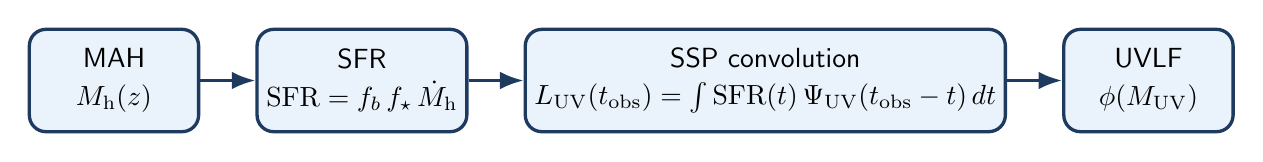
\begin{tikzpicture}[
  node distance=0.9cm and 0.7cm,
  box/.style={draw=MainBlue, very thick, rounded corners=6pt, fill=SoftBlue,
    minimum width=2.15cm, minimum height=1.30cm, align=center, font=\normalsize},
  arr/.style={-{Latex[length=3mm]}, very thick, draw=MainBlue}
]
  \node[box] (mah) {MAH\\[0.15em]$M_{\rm h}(z)$};
  \node[box, right=of mah] (sfr) {SFR\\[0.15em]${\rm SFR}=f_b\,f_\star\,\dot M_{\rm h}$};
  \node[box, right=of sfr, minimum width=3.70cm] (ssp) {SSP convolution\\[0.15em]$L_{\rm UV}(t_{\rm obs})=\int {\rm SFR}(t)\,\Psi_{\rm UV}(t_{\rm obs}-t)\,dt$};
  \node[box, right=of ssp] (uvlf) {UVLF\\[0.15em]$\phi(M_{\rm UV})$};

  \draw[arr] (mah) -- (sfr);
  \draw[arr] (sfr) -- (ssp);
  \draw[arr] (ssp) -- (uvlf);
\end{tikzpicture}
}

\vspace{0.8em}

\normalsize
MAH 采用 McBride et al. (2009) 参数化，并对 \(\beta,\gamma\) 做 Monte Carlo 采样。

\vspace{0.3em}

\begin{minipage}{0.9\linewidth}
\centering
\large
\[
M_{\rm h}(z)=M_{\rm h,obs}\left(\frac{1+z}{1+z_{\rm obs}}\right)^\beta
\exp\!\left[-\gamma\,(z-z_{\rm obs})\right]
\]
\[
f_\star(M)=\frac{2\epsilon_0}{(M/M_c)^{-\beta_\star}+(M/M_c)^{\gamma_\star}}
\]
\end{minipage}
\end{frame}

\begin{frame}{Intrinsic UVLF：从 halo 样本到 \(\phi(M_{\rm UV})\)}
\begin{columns}[T,onlytextwidth]
  \column{0.53\textwidth}
  \centering
  \resizebox{0.98\linewidth}{!}{
  \begin{tikzpicture}[
    node distance=0.8cm and 0.55cm,
    box/.style={draw=MainBlue, very thick, rounded corners=6pt, fill=SoftOrange,
      minimum width=2.2cm, minimum height=1.2cm, align=center, font=\normalsize},
    arr/.style={-{Latex[length=2.8mm]}, very thick, draw=MainBlue}
  ]
    \node[box] (hmf) {HMF 抽样\\$M_{{\rm h},i}$};
    \node[box, right=of hmf] (tracks) {每个质量抽\\\(n_{\rm tracks}\) 条轨道};
    \node[box, right=of tracks] (muv) {得到样本\\$M_{{\rm UV},ij}^{\rm int}$};
    \node[box, right=of muv] (hist) {加权 histogram\\$\phi(M_{\rm UV})$};

    \draw[arr] (hmf) -- (tracks);
    \draw[arr] (tracks) -- (muv);
    \draw[arr] (muv) -- (hist);
  \end{tikzpicture}
  }

  \vspace{1.0em}

  \small
  \begin{itemize}
    \item 外层按 HMF 抽样终质量 \(M_{{\rm h},i}\)
    \item 内层对每个质量生成 \(n_{\rm tracks}\) 条 MAH realization
    \item 最后按 intrinsic \(M_{\rm UV}\) 分 bin，而不是按质量分 bin
  \end{itemize}

  \column{0.44\textwidth}
  \footnotesize
  \begin{align*}
  w_i
  &= \frac{\log M_{\max}-\log M_{\min}}{N_{\rm mass}}
  \left.\frac{dn}{d\log M}\right|_{M_{{\rm h},i}}
  \end{align*}

  \begin{align*}
  w_{ij} &= \frac{w_i}{n_{\rm tracks}}
  \end{align*}

  \begin{align*}
  \phi(M_k)
  &= \frac{1}{\Delta M_k}
  \sum_{ij\in k} w_{ij}
  \end{align*}

  \begin{align*}
  \phi(M_{\rm UV})
  &= \int d\log M_{\rm h}\,
  \frac{dn}{d\log M_{\rm h}} \\
  &\quad \times P(M_{\rm UV}\mid M_{\rm h},z)
  \end{align*}

  \vspace{0.4em}
  \normalsize
  \textbf{这一页讨论的是 intrinsic UVLF，尚未加入 dust。}
\end{columns}
\end{frame}

\begin{frame}{Intrinsic UVLF 的 halo 质量组成：\(z=6,8\)}
\begin{columns}[T,onlytextwidth]
  \column{0.49\textwidth}
  \centering
  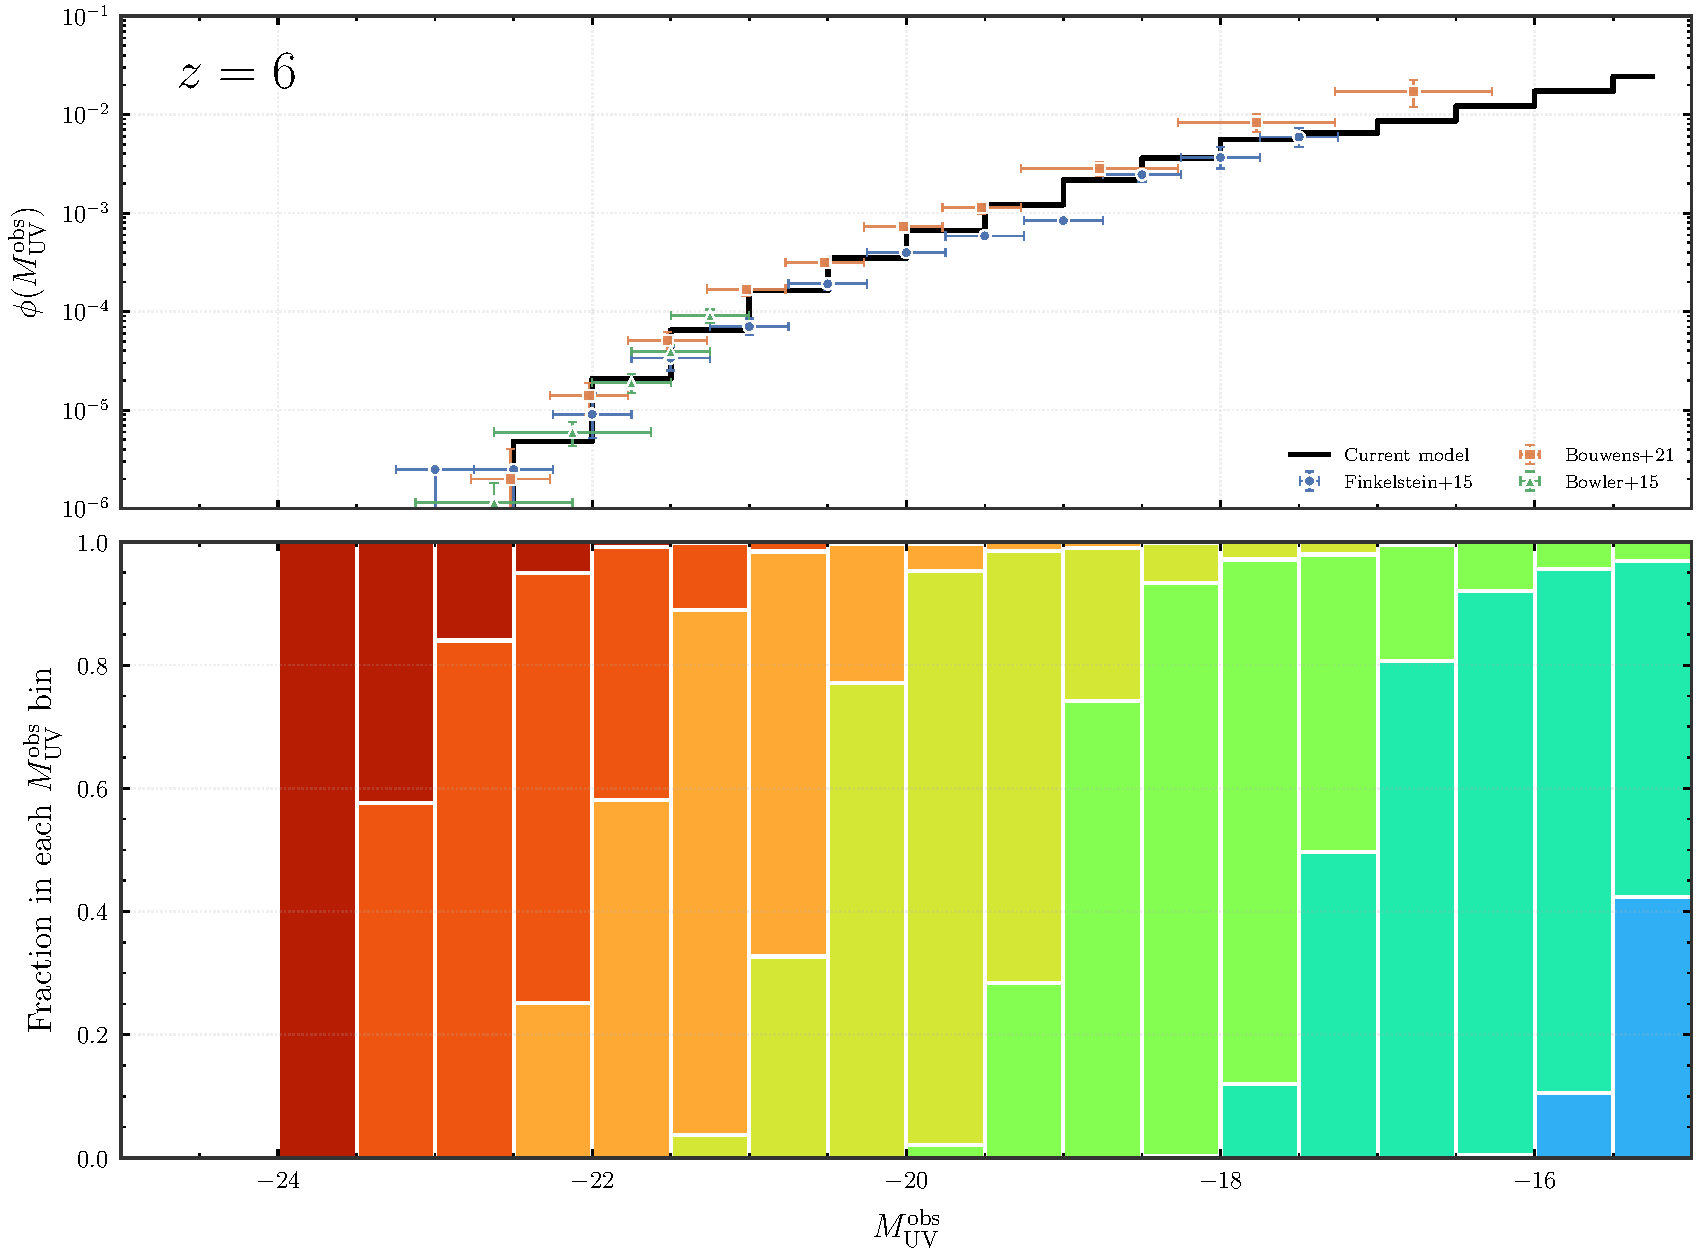
\includegraphics[width=0.98\linewidth,height=0.74\textheight,keepaspectratio]{uvlf_full_mass_composition_z6_m25_m15.pdf}

  \vspace{0.2em}
  {\large \(z=6\)}

  \column{0.49\textwidth}
  \centering
  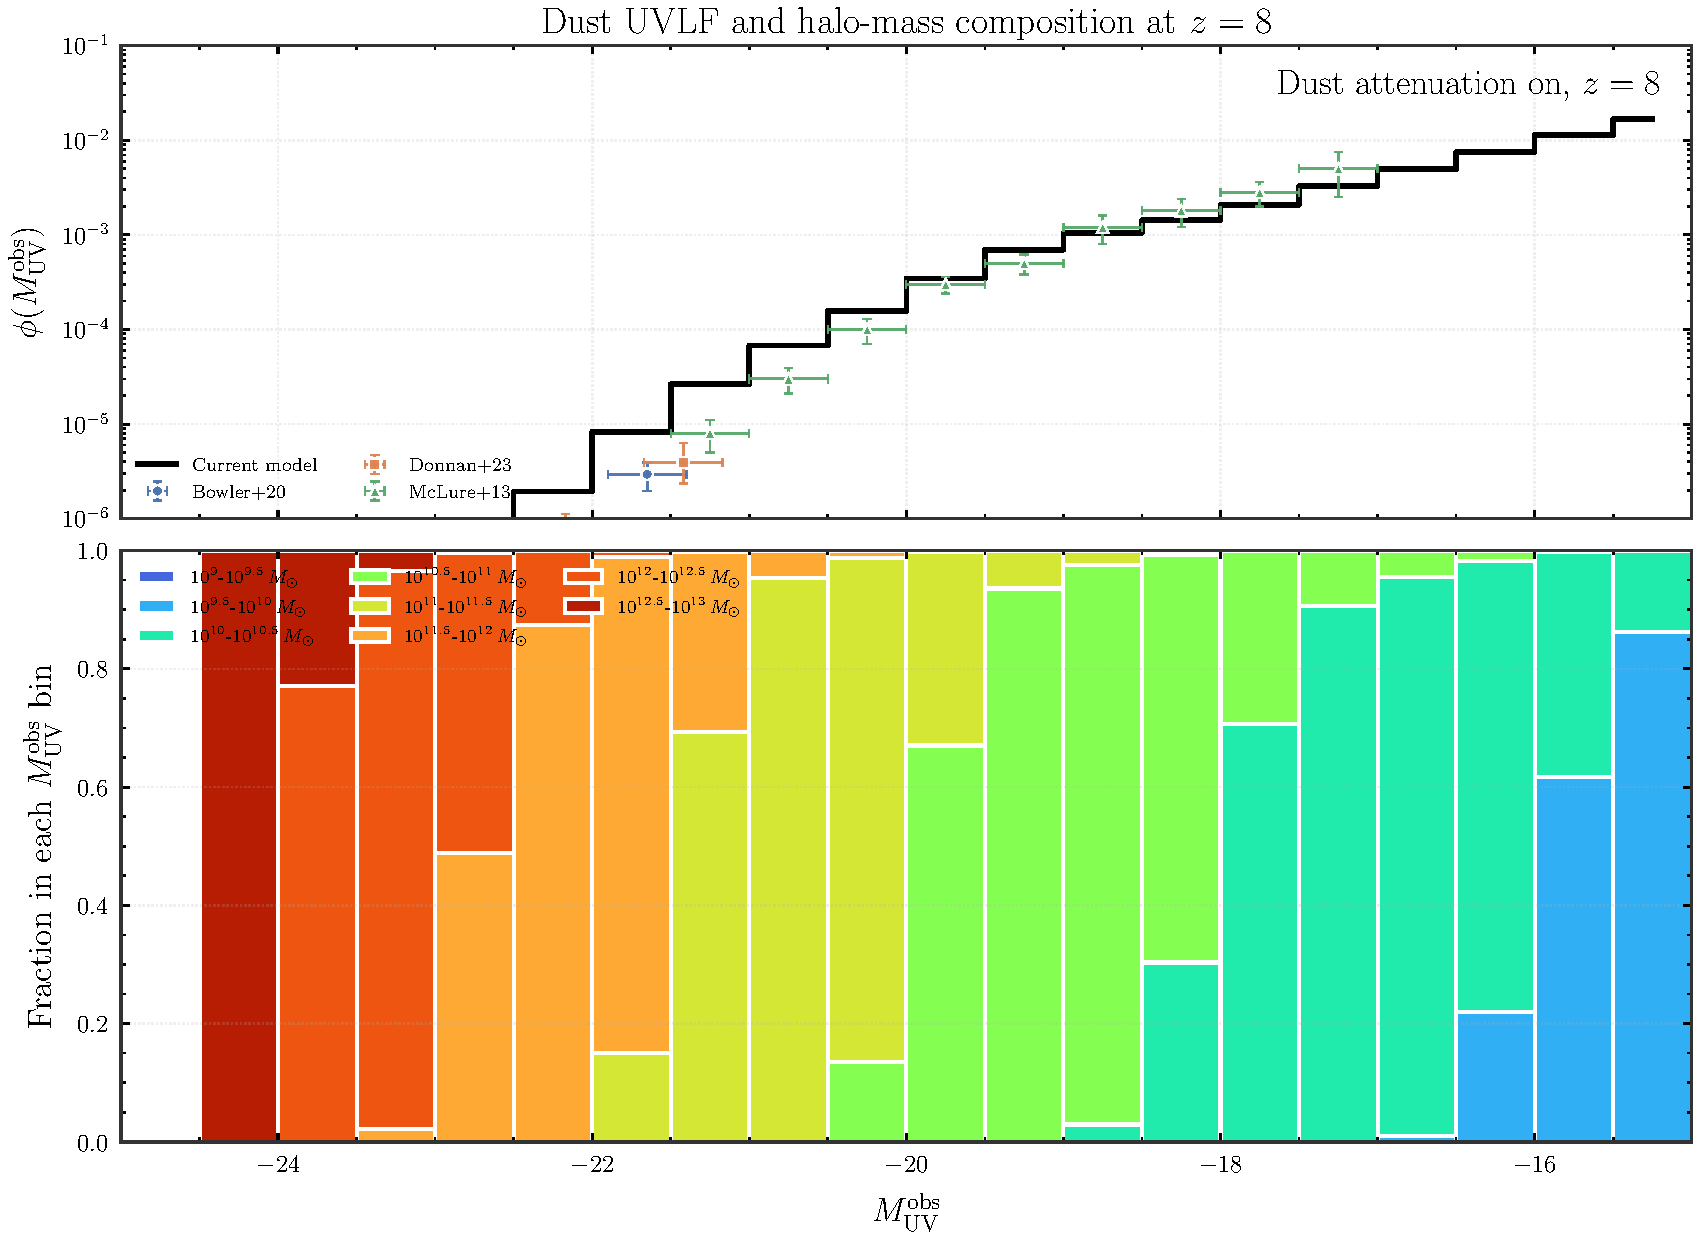
\includegraphics[width=0.98\linewidth,height=0.74\textheight,keepaspectratio]{uvlf_full_mass_composition_z8_m25_m15.pdf}

  \vspace{0.2em}
  {\large \(z=8\)}
\end{columns}
\end{frame}

\begin{frame}{Intrinsic UVLF 的 halo 质量组成：\(z=10,12.5\)}
\begin{columns}[T,onlytextwidth]
  \column{0.49\textwidth}
  \centering
  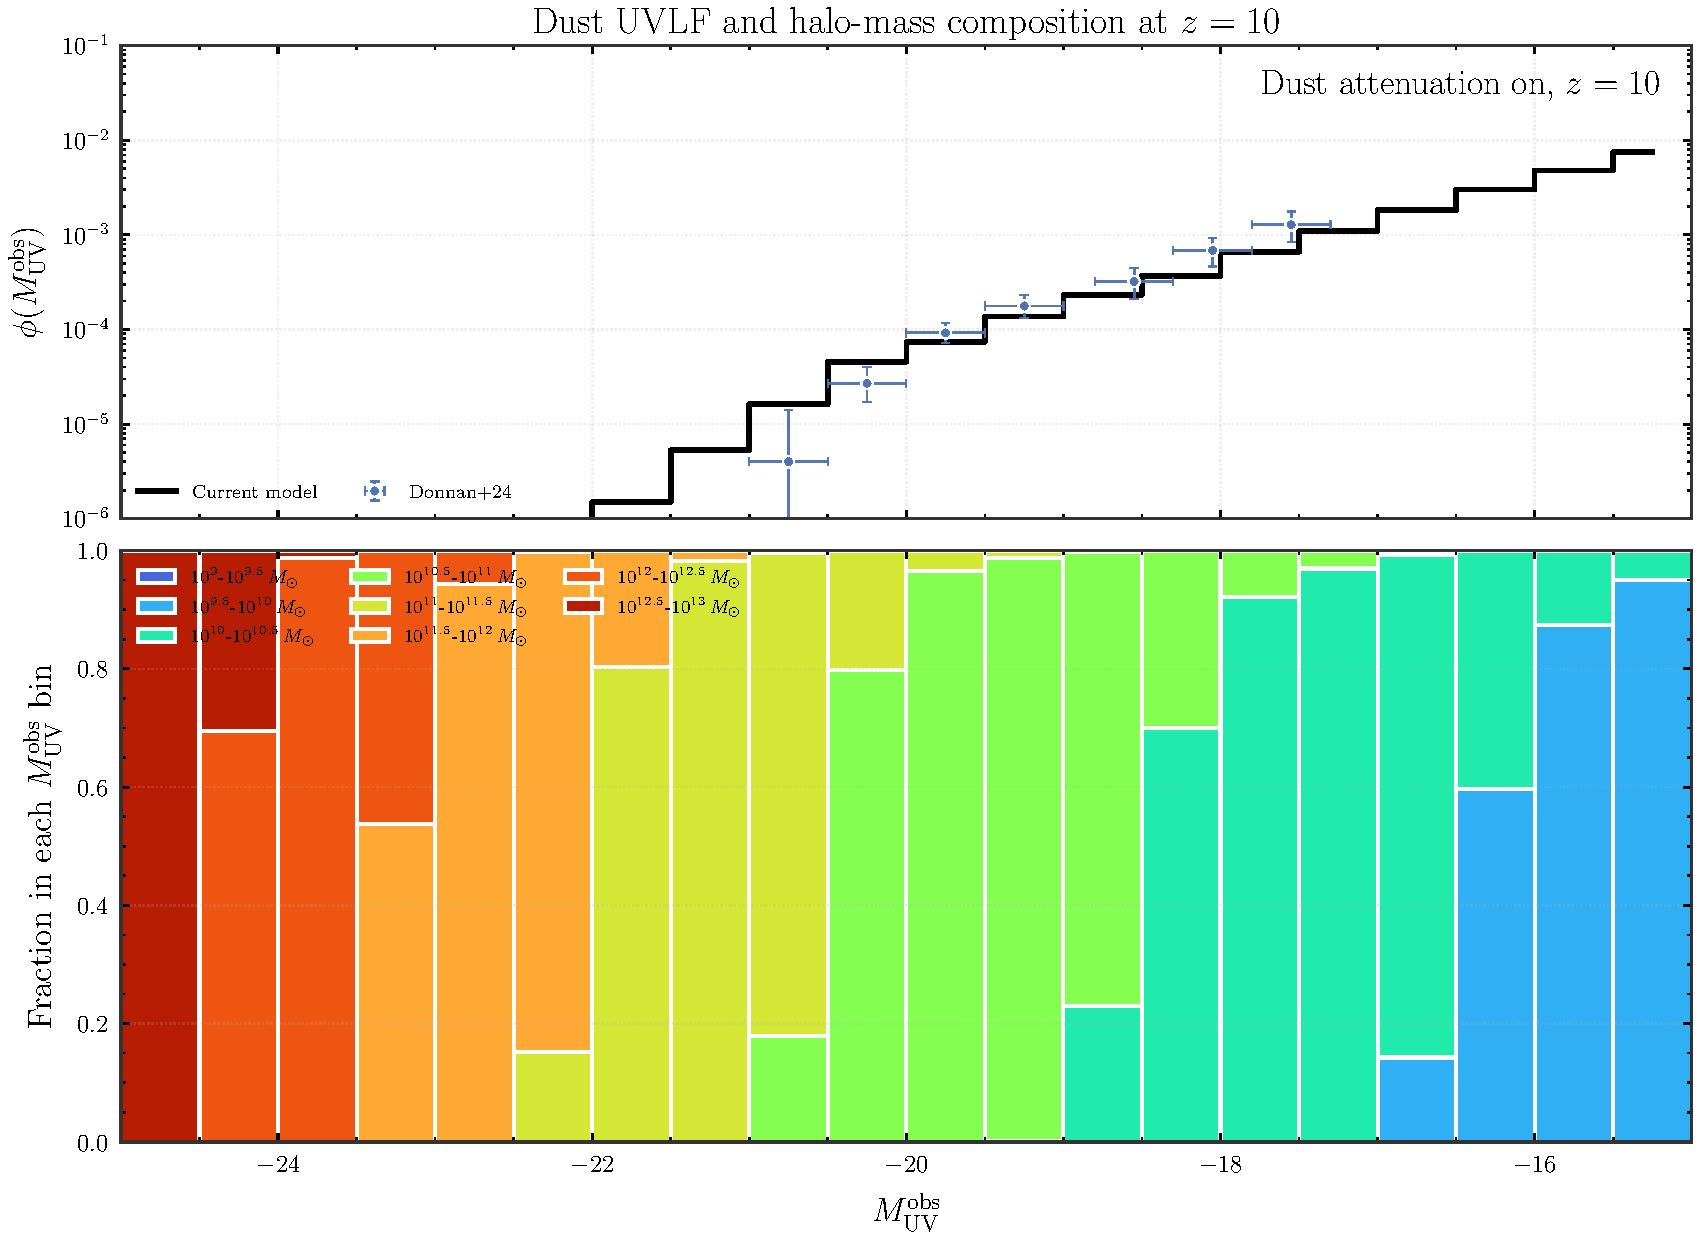
\includegraphics[width=0.98\linewidth,height=0.74\textheight,keepaspectratio]{uvlf_full_mass_composition_z10_m25_m15.pdf}

  \vspace{0.2em}
  {\large \(z=10\)}

  \column{0.49\textwidth}
  \centering
  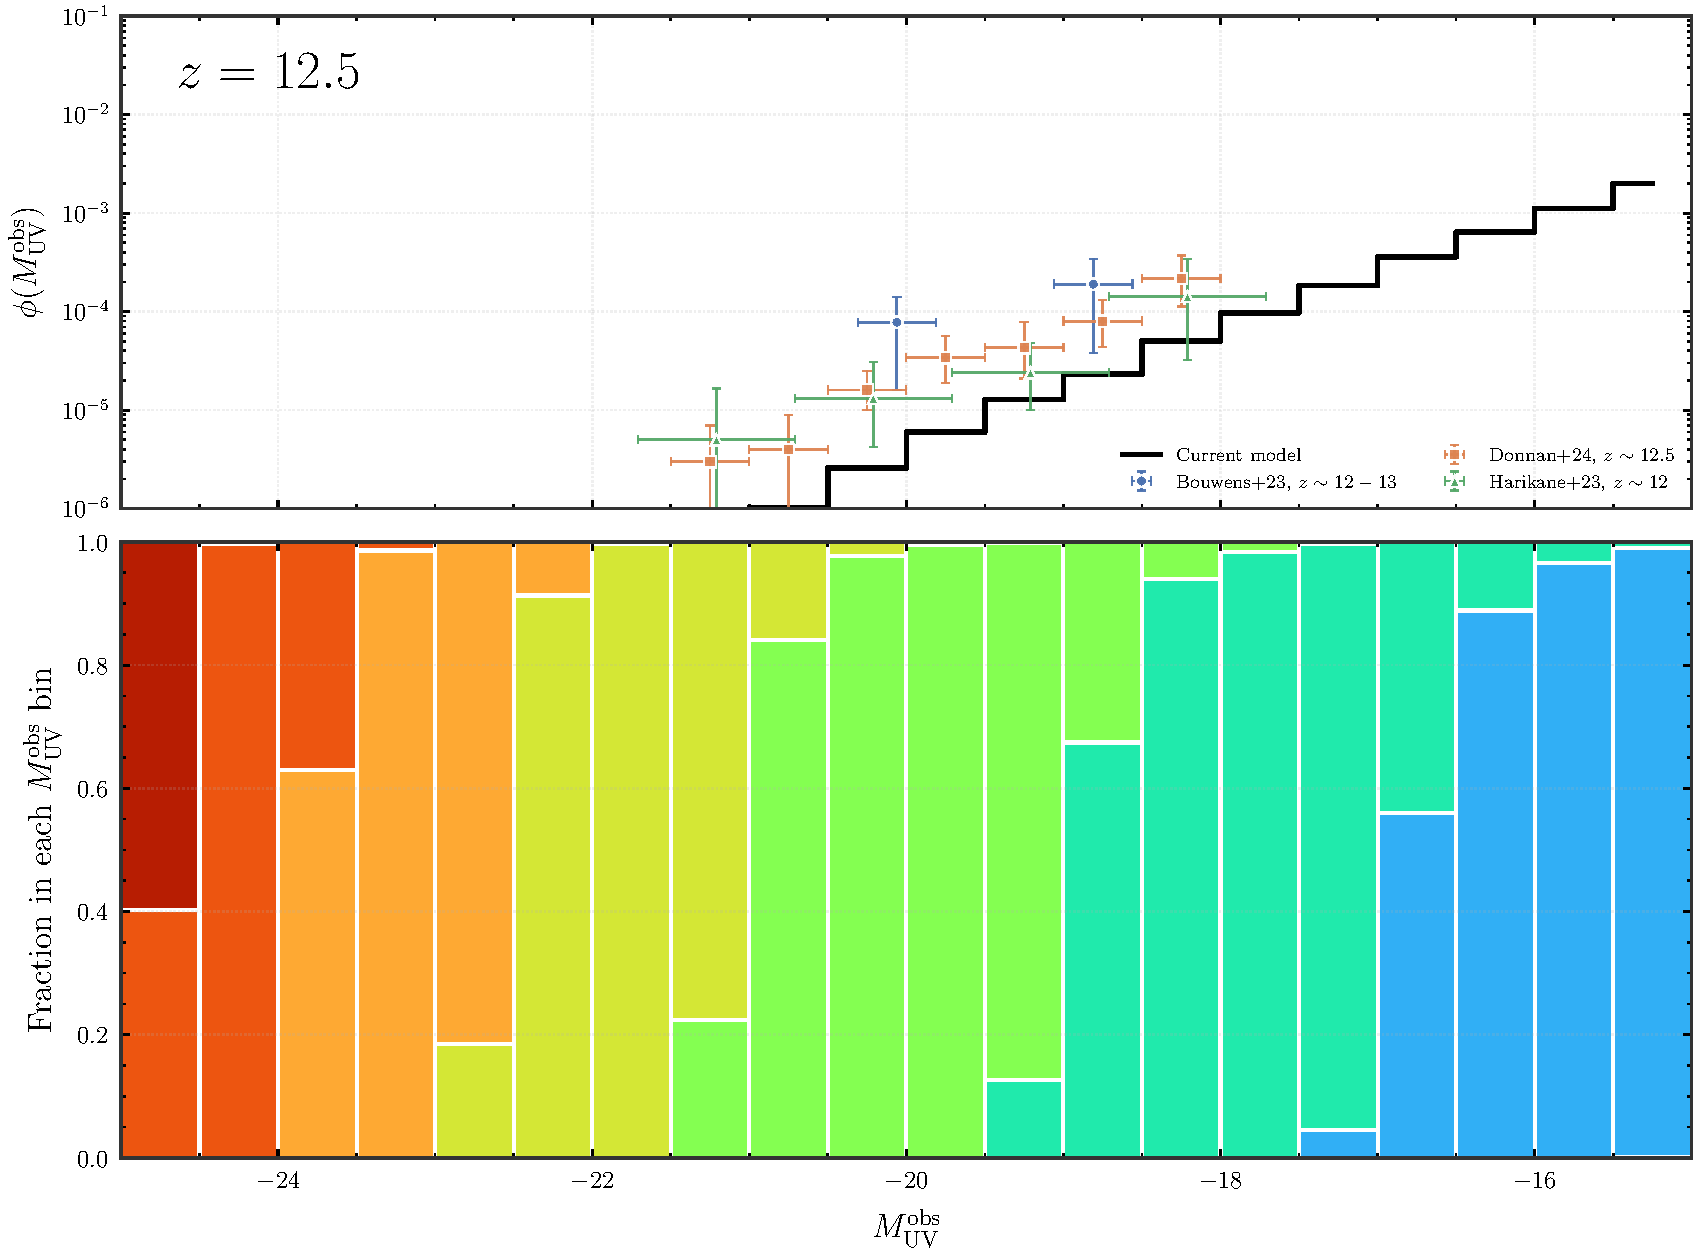
\includegraphics[width=0.98\linewidth,height=0.74\textheight,keepaspectratio]{uvlf_full_mass_composition_z12p5_m25_m15.pdf}

  \vspace{0.2em}
  {\large \(z=12.5\)}
\end{columns}
\end{frame}

\begin{frame}{质量抽样范围的结论}
\begin{beamercolorbox}[rounded=true, sep=0.8em, wd=0.92\linewidth, center]{block body}
\large
\textbf{根据四个红移的 halo 质量组成图，当前观测相关区间}
\[
M_{\rm UV}\in[-25,-15]
\]
\textbf{的主要贡献几乎全部来自}
\[
10^{9} \lesssim M_{\rm h}/M_\odot \lesssim 10^{13}.
\]
\end{beamercolorbox}

\vspace{0.8em}

\begin{beamercolorbox}[rounded=true, sep=0.65em, wd=0.92\linewidth]{block body}
\normalsize
\textbf{计算上的含义}

\vspace{0.25em}
\begin{itemize}
\item HMF 抽样范围取 \(10^9\)–\(10^{13}\,M_\odot\) 已足够。
\item \(M_{\rm h}<10^9\,M_\odot\) 与 \(M_{\rm h}>10^{13}\,M_\odot\) 对当前 UVLF 贡献都可忽略。
\end{itemize}
\end{beamercolorbox}
\end{frame}

\begin{frame}{同参数对比：\(z=6,8\)}
\begin{columns}[T,onlytextwidth]
  \column{0.5\textwidth}
  \centering
  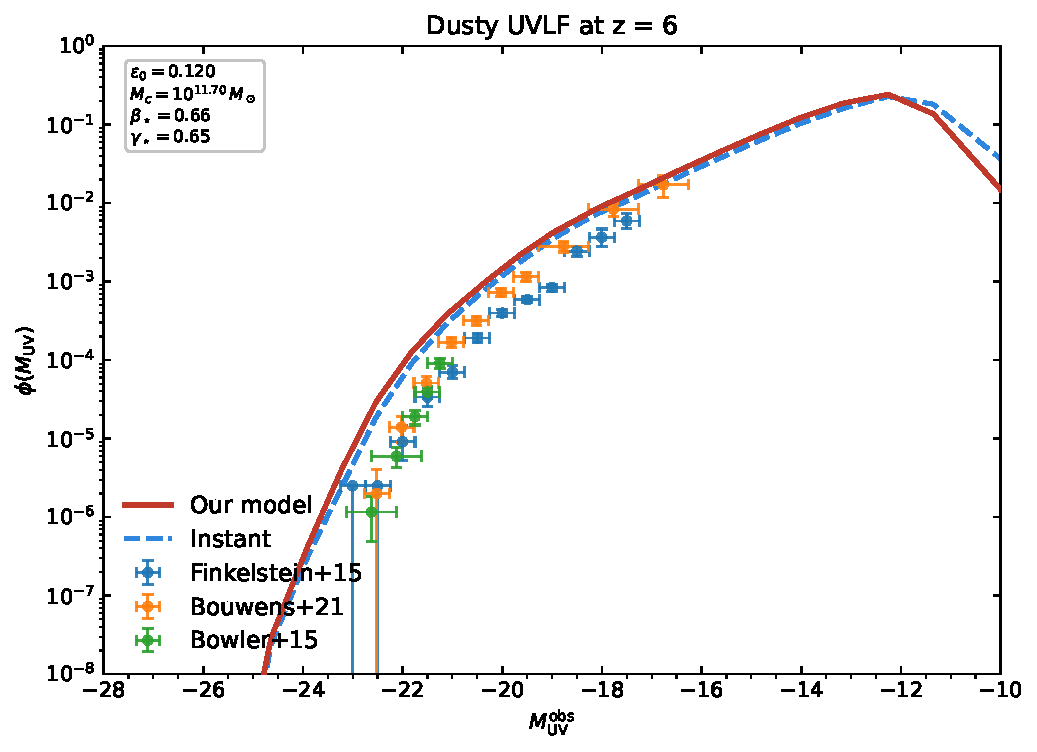
\includegraphics[width=0.97\linewidth]{uvlf_compare_no_puv_z6_dustonly.pdf}
  \vspace{-0.5em}
  {\large \(z=6\)}

  \column{0.5\textwidth}
  \centering
  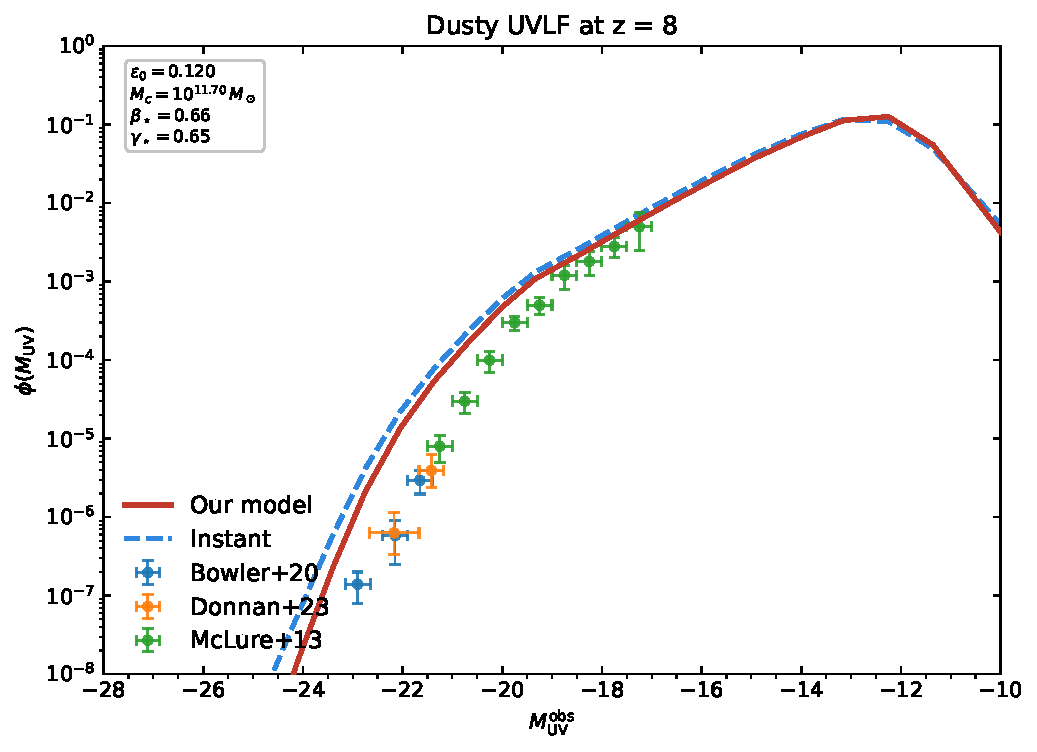
\includegraphics[width=0.97\linewidth]{uvlf_compare_no_puv_z8_dustonly.pdf}
  \vspace{-0.5em}
  {\large \(z=8\)}
\end{columns}
\end{frame}

\begin{frame}{同参数对比：\(z=10,12.5\)}
\begin{columns}[T,onlytextwidth]
  \column{0.5\textwidth}
  \centering
  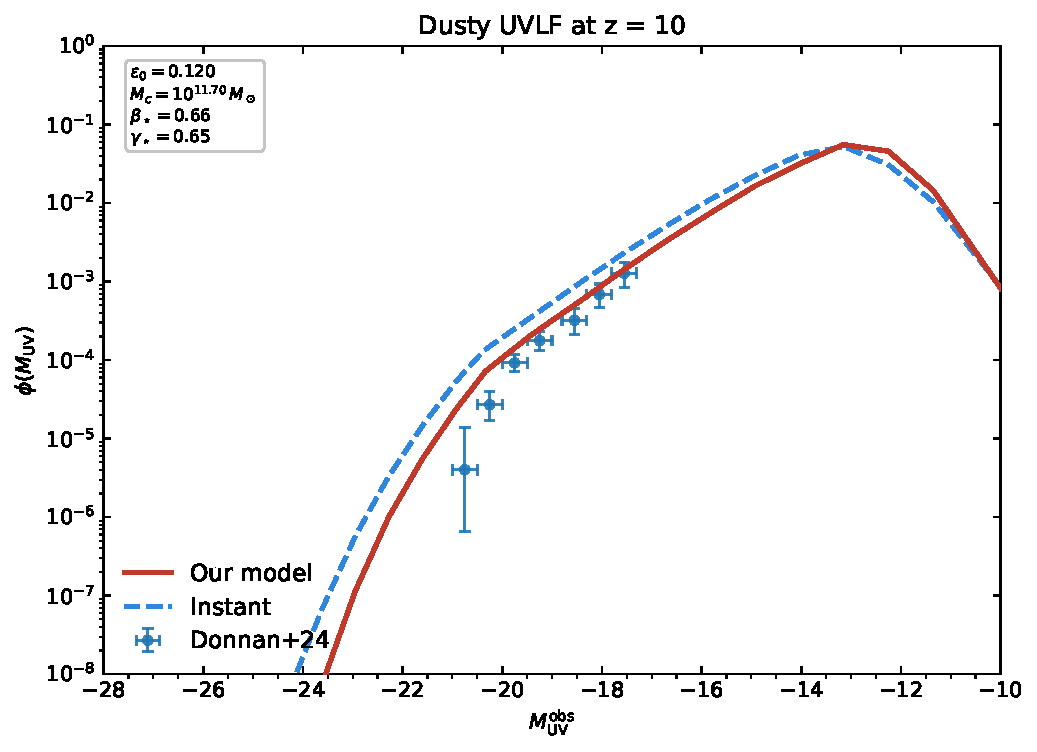
\includegraphics[width=0.97\linewidth]{uvlf_compare_no_puv_z10_dustonly.pdf}
  \vspace{-0.5em}
  {\large \(z=10\)}

  \column{0.5\textwidth}
  \centering
  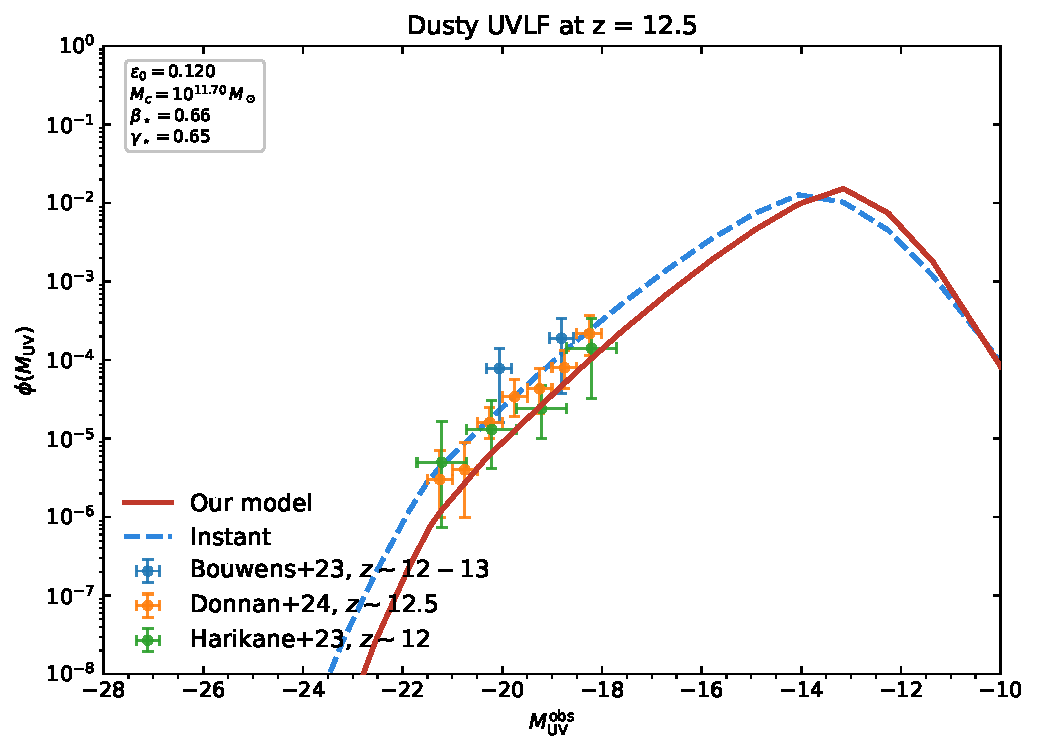
\includegraphics[width=0.97\linewidth]{uvlf_compare_no_puv_z12p5_dustonly.pdf}
  \vspace{-0.5em}
  {\large \(z=12.5\)}
\end{columns}
\end{frame}

\begin{frame}{Why Add A Delay Kernel?}
\begin{columns}[T,onlytextwidth]
  \column{0.52\textwidth}
  \large
  \begin{itemize}
    \item 现在的 SFR 若直接取
    \[
    \mathrm{SFR}\propto f_\star(M_{\rm h})\,\dot M_{\rm h},
    \]
    等价于假设新吸积 gas 立刻形成恒星
    \item 这会把 star formation 与瞬时 accretion 绑定得过紧
    \item 但实际 gas cooling、collapse、feedback 都会引入有限时间延迟
  \end{itemize}

  \column{0.44\textwidth}
  \begin{beamercolorbox}[rounded=true, sep=0.85em, wd=\linewidth]{block body}
  \large
  引入 delay kernel 的目的：

  \vspace{0.5em}
  \begin{itemize}
    \item 把瞬时吸积率平滑成有限时宽的 SFR 响应
    \item 让模型从 instantaneous burst 变成 extended burst
    \item 用一个参数 \(\kappa\) 控制时间尺度
  \end{itemize}
  \end{beamercolorbox}
\end{columns}
\end{frame}

\begin{frame}{Delayed Star Formation Kernel}
\begin{columns}[T,onlytextwidth]
  \column{0.40\textwidth}
  \footnotesize
  \[
  \dot M_{{\rm h},{\rm burst}}(t)
  =
  \int_{t-\Delta t_{\max}}^{t}
  g(t-t')\,\dot M_{\rm h}(t')\,dt'
  \]

  \[
  g(t-t')
  =
  \frac{t-t'}{\kappa^2 t_d^2(z_f)}
  \exp\!\left[-\frac{t-t'}{\kappa t_d(z_f)}\right]
  \]

  \[
  t_d(z_f)
  =
  \sqrt{\frac{3\pi}{32G\,\rho_{\rm vir}(z_f)}}
  \]

  \[
  \mathrm{SFR}(t)
  =
  f_b\,f_\star\!\bigl(M_{\rm h}(t)\bigr)\,
  \dot M_{{\rm h},{\rm burst}}(t)
  \]

  \vspace{0.35em}
  \begin{beamercolorbox}[rounded=true, sep=0.6em, wd=\linewidth]{block body}
  \footnotesize
  我们取
  \[
  \kappa = 0.1
  \]
  {\scriptsize Yue et al.\ (2016), MNRAS, 463, 1968}
  \end{beamercolorbox}

  \column{0.57\textwidth}
  \centering
  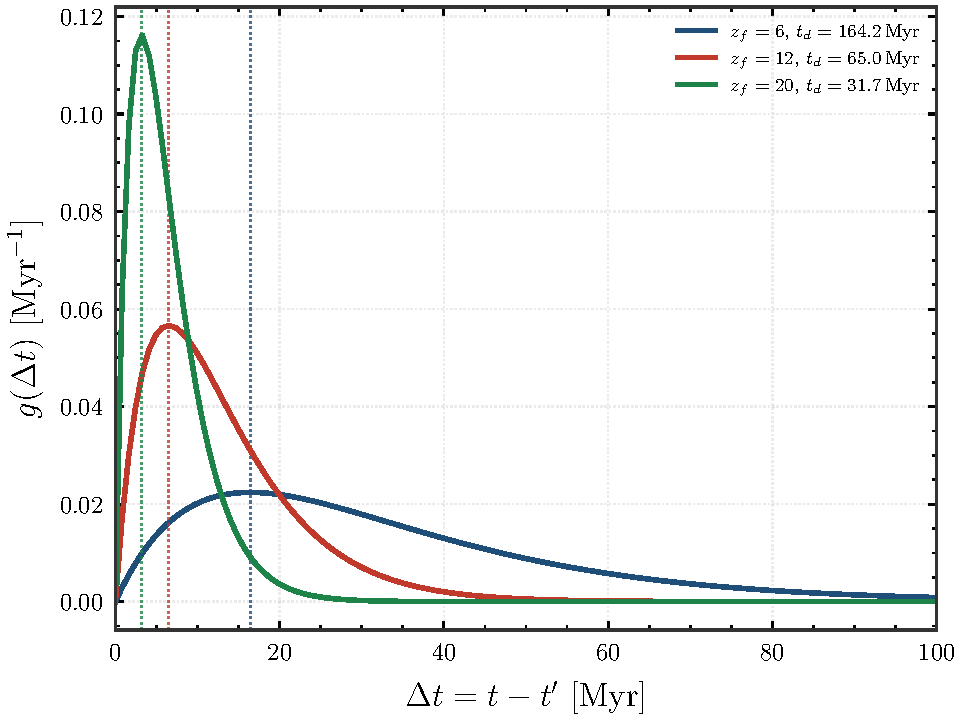
\includegraphics[width=\linewidth]{extended_burst_kernel_kappa0p1_xmax100.pdf}
\end{columns}
\end{frame}

\begin{frame}{Delayed SFR}
\footnotesize
\begin{columns}[T,onlytextwidth]
  \column{0.52\textwidth}
  \begin{align*}
  f_\star(M)
  &= \frac{2\epsilon_0}
  {(M/M_c)^{-\beta_\star} + (M/M_c)^{\gamma_\star}}
  \end{align*}

  \[
  {\rm SFR}(t_i)=
  \begin{cases}
  \dfrac{f_b}{10^9}
  \int_0^{100~{\rm Myr}} g(\Delta t)\,
  f_\star[M_{\rm h}(t_i-\Delta t)] \\
  \qquad\qquad \times \dot M_{\rm h}(t_i-\Delta t)\,d\Delta t, \\
  \hfill T_{\rm vir}(t_i)\ge 10^4~{\rm K} \\
  0,\qquad\text{otherwise}
  \end{cases}
  \]
  {\scriptsize 这里的 \(10^9\) 只是把 Gyr 换成 yr。}

  \column{0.42\textwidth}
  \begin{beamercolorbox}[rounded=true, sep=0.7em, wd=\linewidth]{block body}
  \footnotesize
  \textbf{实现口径}

  \vspace{0.25em}
  对每条 halo 的 \(M_{\rm h}(t)\)，在最近
  \(100\,{\rm Myr}\) 的因果区间内，把
  \(f_\star[M_{\rm h}(t)]\,\dot M_{\rm h}(t)\)
  与 delay kernel 做卷积，得到 delayed SFR。
  \end{beamercolorbox}

  \vspace{0.45em}
  \begin{beamercolorbox}[rounded=true, sep=0.7em, wd=\linewidth]{block body}
  \footnotesize
  \textbf{100 Myr 截断诊断}

  \vspace{0.25em}
  固定 \(M_{\rm h,final}=10^{11}M_\odot\) 时，
  在 \(t_i=t_{\rm obs}\) 比较
  \[
  {\rm median}\!\left(
  \frac{{\rm SFR}_{\Delta t_{\max}=100\,{\rm Myr}}}
  {{\rm SFR}_{\Delta t_{\max}=1000\,{\rm Myr}}}
  \right)
  \]

  \vspace{0.2em}
  把 \(1000\,{\rm Myr}\) 视为近似收敛值，则
  \(z=6,8,10,12.5\) 时中位数都约为

  \[
  100.0\%
  \]
  最大逐轨偏差也仅约为 \(0.004\%\)。
  \end{beamercolorbox}
\end{columns}
\end{frame}

\begin{frame}{Delay 对 SFR 历史的影响：\(z=6,8\)}
\centering
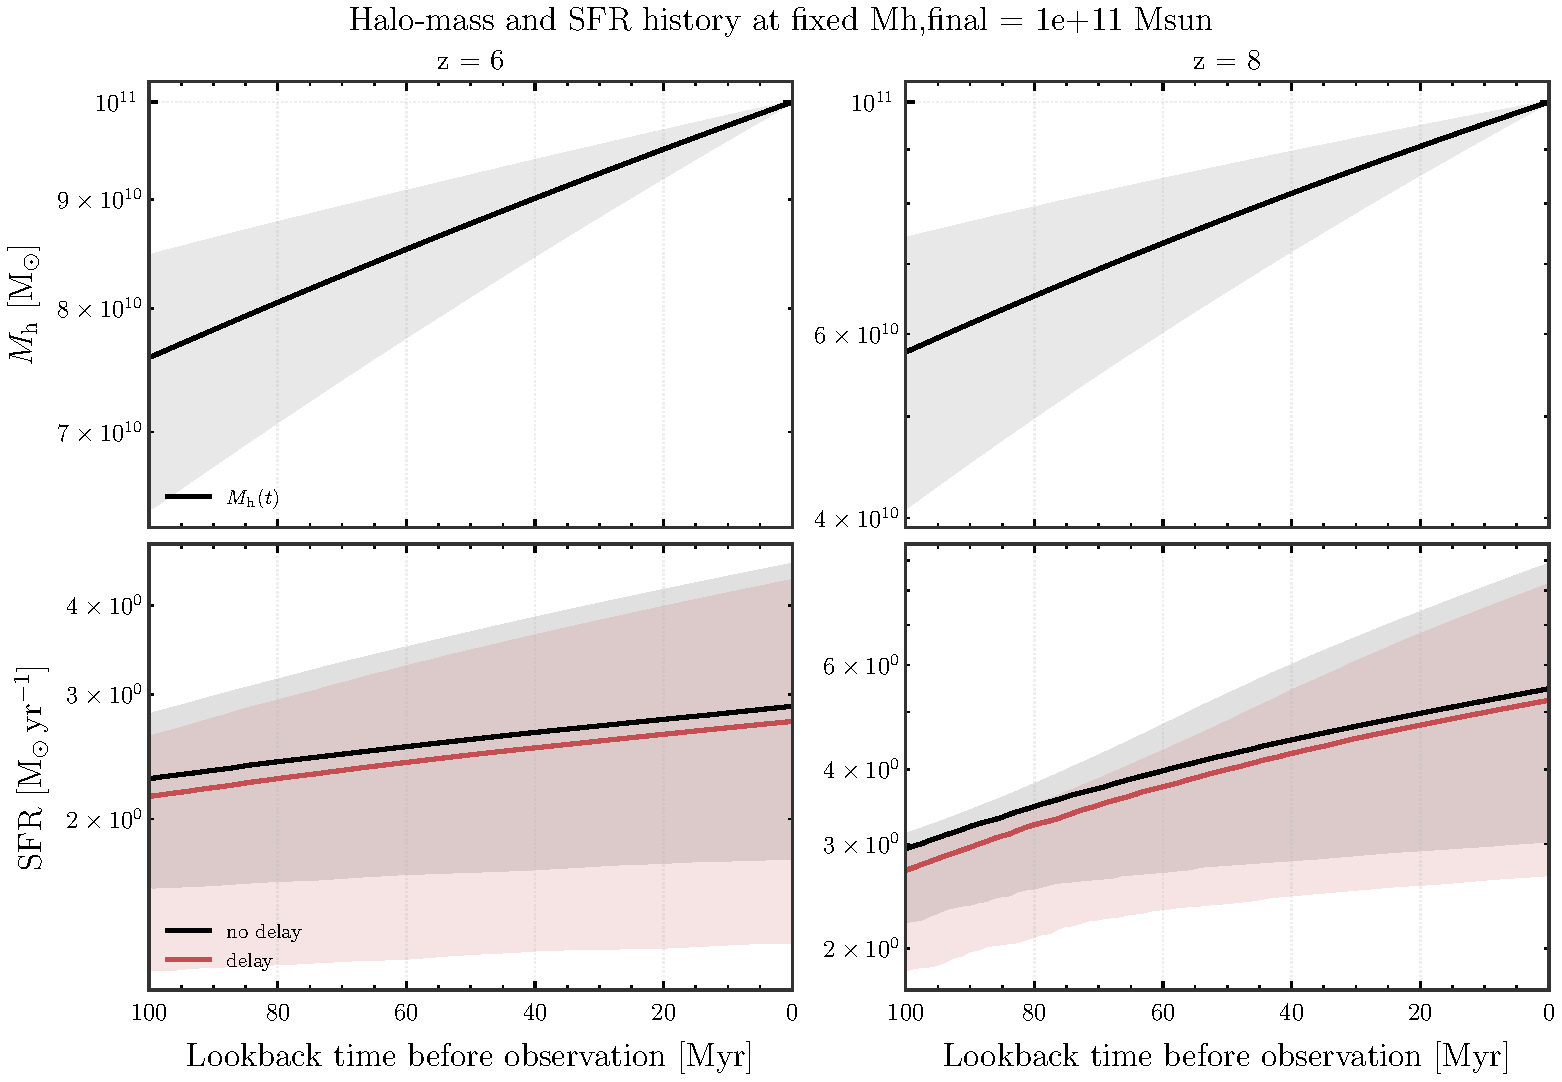
\includegraphics[height=0.74\textheight,keepaspectratio]{assets/delay_sfr_mh_z6_z8.pdf}

\vspace{0.3em}
{\footnotesize 固定 \(M_{\rm h,final}=10^{11}M_\odot\)；上排是同一批 halo 的 \(M_{\rm h}(t)\)，下排比较 delay / no-delay 的 SFR history。}
\end{frame}

\begin{frame}{Delay 对 SFR 历史的影响：\(z=10,12.5\)}
\centering
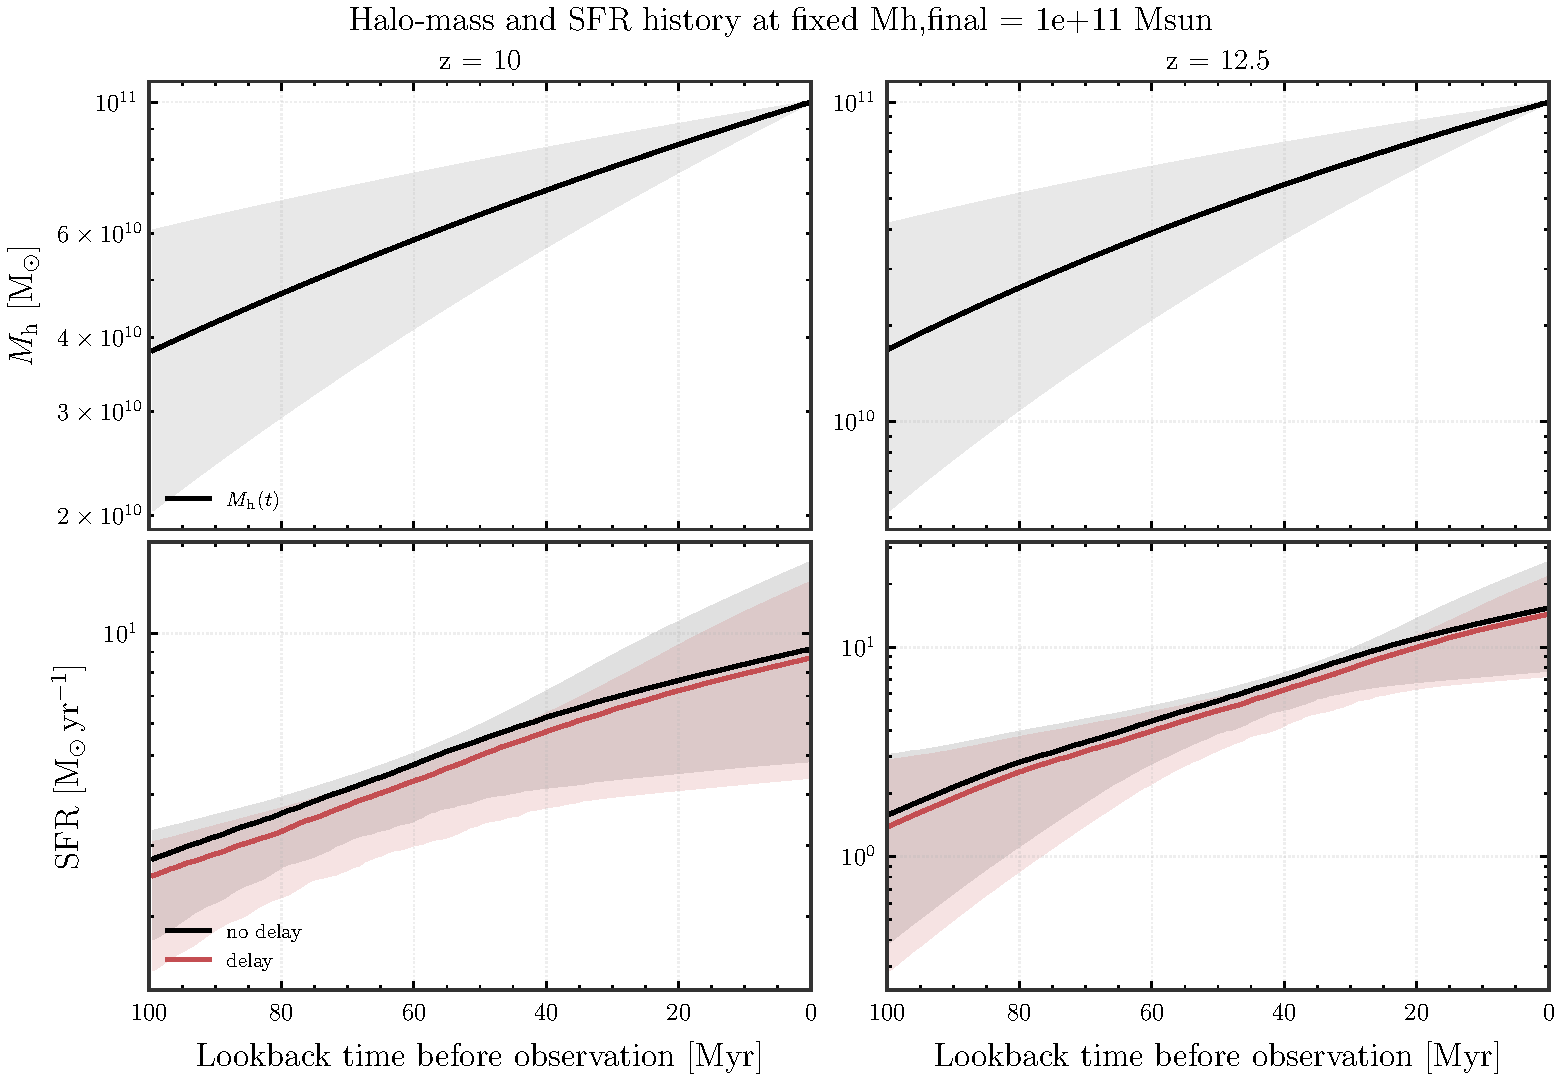
\includegraphics[height=0.74\textheight,keepaspectratio]{assets/delay_sfr_mh_z10_z12p5.pdf}

\vspace{0.3em}
{\footnotesize 高红移时 \(M_{\rm h}(t)\) 在最近 \(100\,{\rm Myr}\) 内下降更快，因此同样的 delay kernel 会带来更明显的 SFR suppression。}
\end{frame}

\begin{frame}{Top-heavy IMF + dust：\(z=6,8\)}
\vspace{-1.85em}
\setlength{\columnsep}{0.028\textwidth}
\begin{columns}[T,onlytextwidth]
  \column{0.495\textwidth}
  \centering
  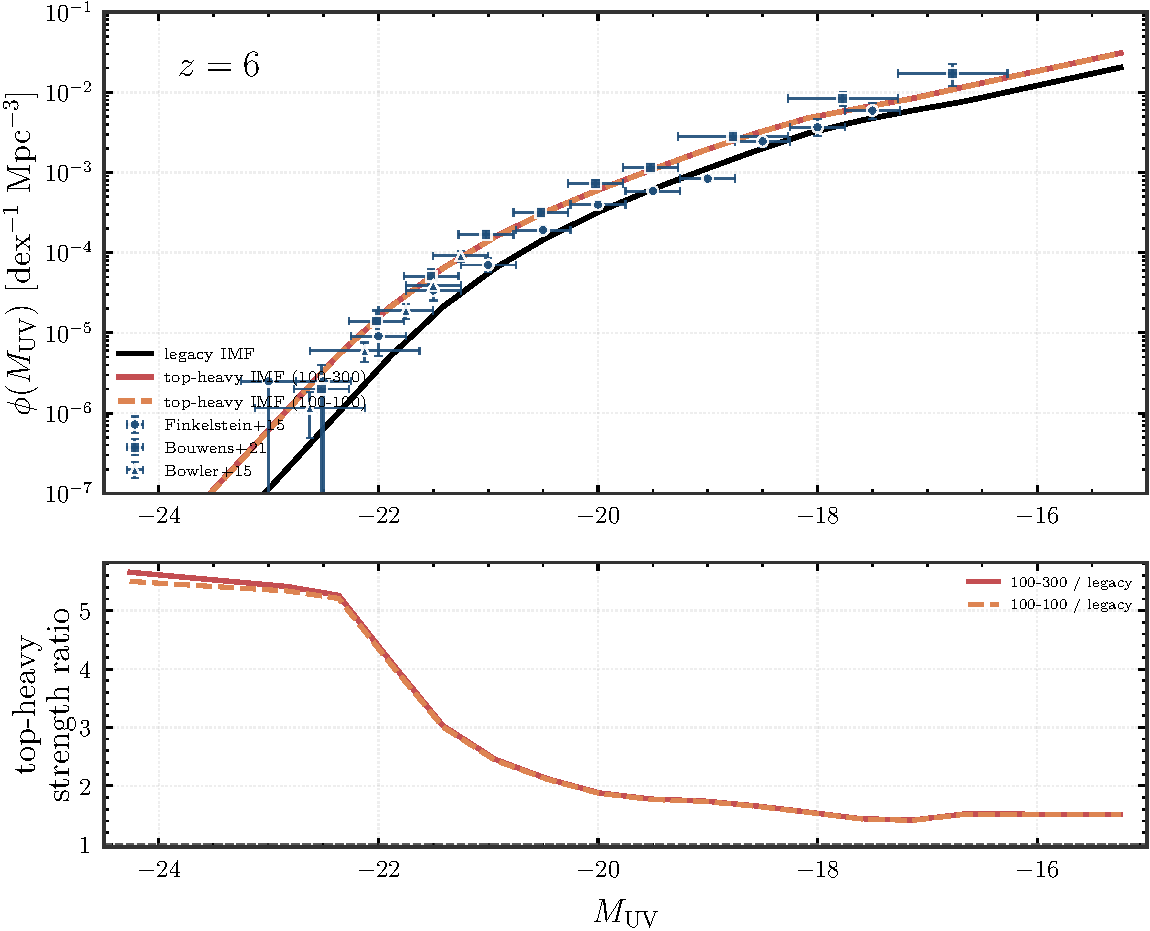
\includegraphics[width=\linewidth]{assets/uvlf_imf_dust_eps005_z6p0.pdf}

  \column{0.495\textwidth}
  \centering
  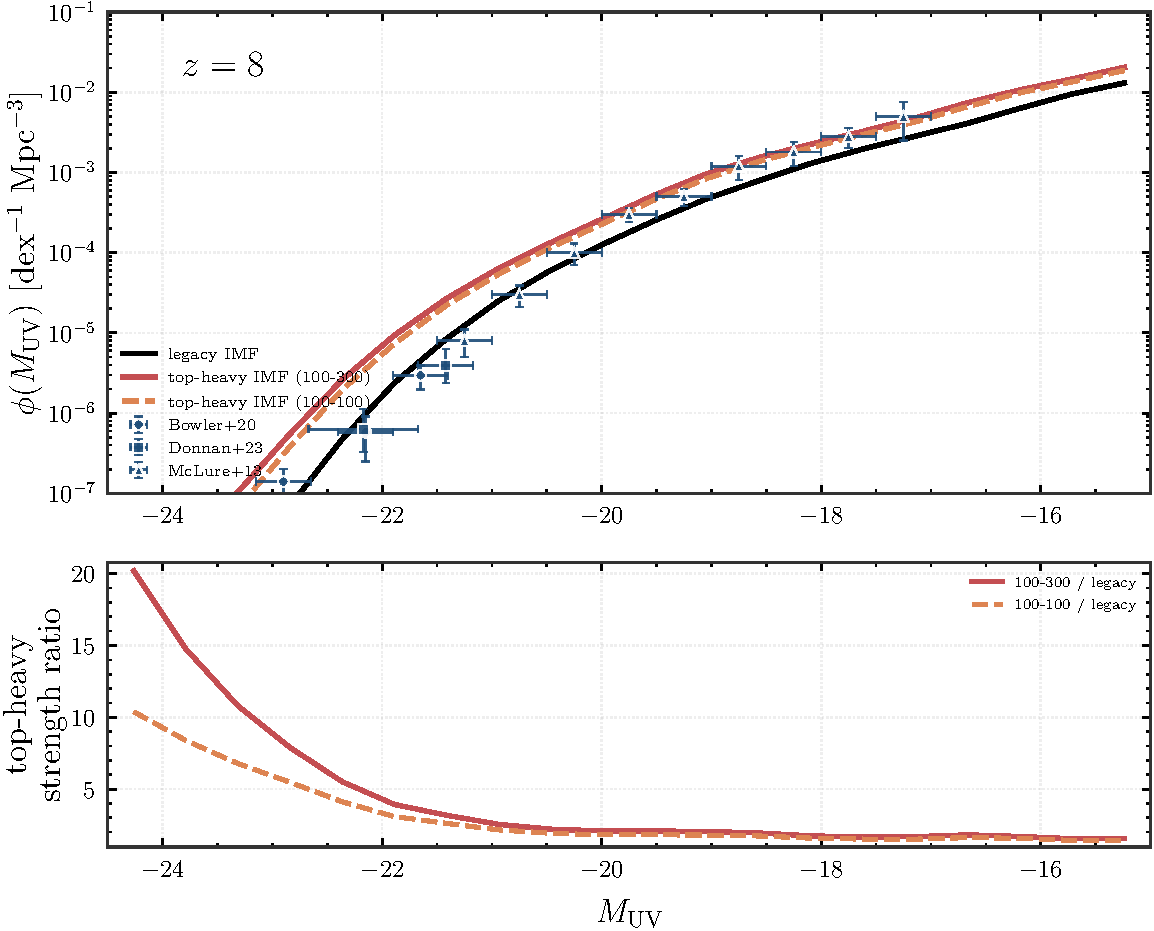
\includegraphics[width=\linewidth]{assets/uvlf_imf_dust_eps005_z8p0.pdf}
\end{columns}
\end{frame}

\begin{frame}{Top-heavy IMF + dust：\(z=10,12.5\)}
\vspace{-1.45em}
\setlength{\columnsep}{0.028\textwidth}
\begin{columns}[T,onlytextwidth]
  \column{0.495\textwidth}
  \centering
  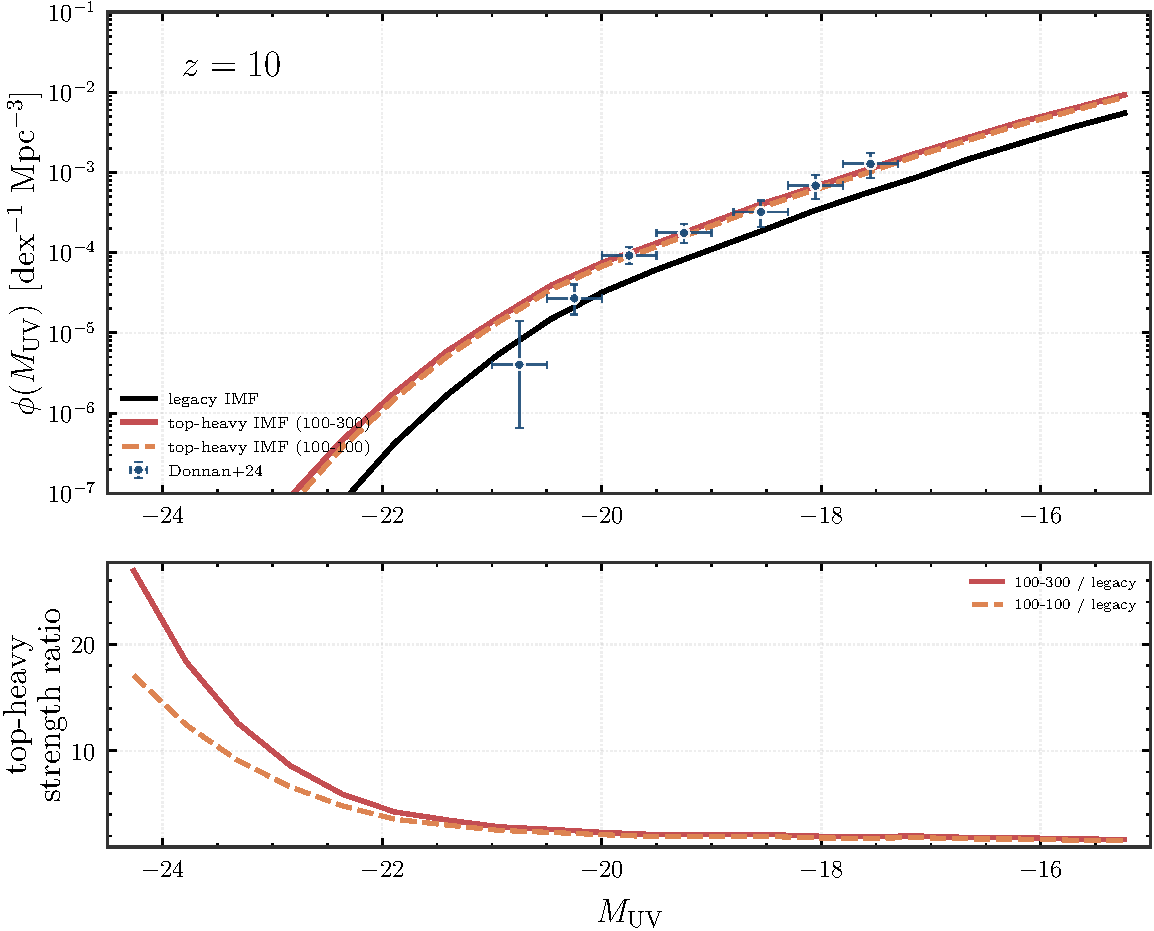
\includegraphics[width=\linewidth]{assets/uvlf_imf_dust_eps005_z10p0.pdf}

  \column{0.495\textwidth}
  \centering
  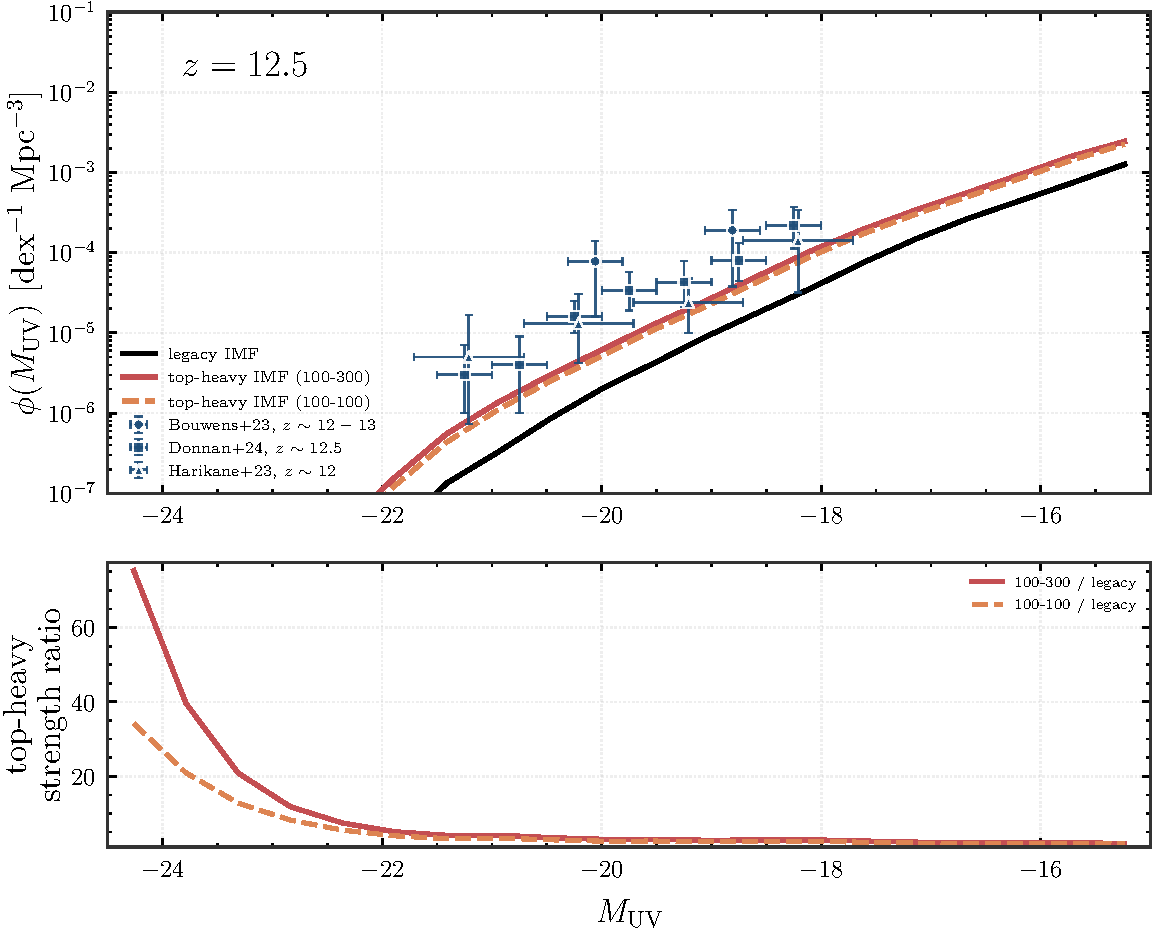
\includegraphics[width=\linewidth]{assets/uvlf_imf_dust_eps005_z12p5.pdf}
\end{columns}

\vspace{0.22em}
{\footnotesize 同一套 dust 口径下，亮端 IMF 差异随 redshift 增强更明显。}
\end{frame}

\end{document}
